\documentclass{report}

\begin{document}
\chapter{Инфологическое проектирование модели базы данных}

\section{Описание сущностей предметной области}
Опишем сущности, выявленные в ходе анализа предметной области.

\textbf{Автоматическая телефонная станция (АТС)}. У АТС имеется 
организация-владелец, первый и последний доступные номера телефонов, 
т.е. диапозон доступных номеров телефонов. 
\newline\textbf{АТС}:
\begin{itemize}
    \item идентификатор
    \item владелец (описательный)
    \item первый телефон (описательный)
    \item последний телефон (описательный)
\end{itemize}
Сущность АТС является супертипом для городской, 
ведомственной и учрежден\-чес\-кой АТС, которые обладают характерным только 
для этой группы, пока неизвестным, набором атрибутов.

В качестве первичного ключа для большинства сущностей будем использовать
отдельный идентификатор, даже когда у нас имеется другой первичный ключ.
Необходимо это для того, чтобы первичный ключ не содержал информацию
о сущности, таким образом мы сможем безболезненно эту информацию
менять. Кроме того, так мы можем избежать состовных ключей для 
сущности имеющей связи.

\textbf{Абонент}. У каждого абонента есть ФИО, 
и следующие атрибуты: пол, возраст, льгота (для подсчета 
абонентской платы), задолжность (для отслеживания долга абонента). 
\newline\textbf{Абонент}:
\begin{itemize}
    \item идентификатор
    \item ФИО (указывающий)
    \item пол (описательный)
    \item возраст (описательный)
    \item льгота (описательный)
    \item задолжность (описательный)
\end{itemize}

\textbf{Номер телефона}. Каждый номер должен принадлежать какой-то АТС, 
чтобы избежать коллизий. Поэтому у номера телефона есть сам номер
и АТС, которой он принадлежит. Кроме того, у телефона есть адрес дома,
в котором он находится (или у которого он находится, в случае таксофона)
\newline\textbf{Номер телефона}:
\begin{itemize}
    \item идентификатор
    \item номер (указывающий)
    \item АТС (вспомогательный)
    \item адрес (описателный)
\end{itemize}
Сущность номер телефона является супертипом для обычного номера, 
которым будет пользоваться абонент, и таксофона, который не принадлежит
никакому абоненту. У обычного номера телефона имеется номер квартиры, 
в которой он находится. 

\textbf{Абонемент}. Абонемент закрепляет обычный номер телефона за абонентом.
Кроме того, абонемент фиксирует тип конечного 
устройства абонента (основной, параллельный, спареный). 
\newline\textbf{Абонемент}:
\begin{itemize}
    \item идентификатор
    \item обычный номер телефона (вспомогательный)
    \item абонент (вспомогательный)
    \item тип телефона (описателный)
\end{itemize}

\textbf{Услуга}. Абонент может подключать различные услуги. Изначально 
каждый абонент может звонить по городу (или ведомству). Далее, если 
ему нужны междугородние звонки или иные функции, он их подлючает. Услуга
характеризуется своим названием и стоимостью.
\newline\textbf{Услуга}:
\begin{itemize}
    \item идентификатор
    \item название (указывающий)
    \item стоимость (описывающий)
\end{itemize}

\textbf{Подключение услуги}. Сущность для связи подключенных услуг с 
абонементом. Подключенная услуга имеет дату последней оплаты, для отслеживания
задолжности. Абонемент и услуга выступают в качестве первичного ключа.
\newline\textbf{Подключение услуги}:
\begin{itemize}
    \item абонемент (вспомогательный)
    \item услуга (вспомогательный)
    \item дата оплаты (описателный)
\end{itemize}

\textbf{Журнал звонков}. Эта сущность необходима для сбора сведений 
о всех произошедших звонках. Любой звонок имеет дату и время начала,
длительность и пункт назначения. Чтобы избежать потери истории звонков, 
здесь не используется сущность Абонемент, 
так как абонент может отказаться от абонемента по разным причинам, 
например если он продал квартиру.
\newline\textbf{Журнал звонков}:
\begin{itemize}
    \item абонент (вспомогательный)
    \item обычный номер телефона (вспомогательный)
    \item дата и время (указывающий)
    \item длительность (описателный)
    \item пункт назначения (описателный)
\end{itemize}

Кроме вышеописанных сущностей нам понадобится сущности предстваляющие карту 
нашего города и информацию о других городах. Кратко опишем их.
\begin{itemize}
    \item[] \textbf{Город}
    \begin{itemize}
        \item идентификатор
        \item название (указывающий)
    \end{itemize}
    \item[] \textbf{Район}
    \begin{itemize}
        \item идентификатор
        \item город (вспомогательный)
        \item название (указывающий)
    \end{itemize} 
    \item[] \textbf{Улица}
    \begin{itemize}
        \item идентификатор
        \item район (вспомогательный)
        \item название (указывающий)
    \end{itemize} 
    \item[] \textbf{Адрес}
    \begin{itemize}
        \item идентификатор
        \item улица (вспомогательный)
        \item номер дома (указывающий)
    \end{itemize} 
\end{itemize}

\section{Описание связей}
\begin{longtblr}[caption = {Описание связей}, theme = TC,]{
        colspec={|X|X[4]|X|X[8]|}, row{1} = {c}, hlines,
    }
    Связь & Сущности & Тип & Описание \\
    R1 & АТС - ведомственная АТС & 1:1 & Связь супертип-подтип \\
    R2 & АТС - учрежденческая АТС & 1:1 & Связь супертип-подтип \\
    R3 & АТС - городская АТС & 1:1 & Связь супертип-подтип \\
    R4 & АТС - номер телефона & 1:M & 
        К АТС подключено множество номеров. У каждого номера только одна АТС \\
    R5 & Номер телефона - обычный номер телефона & 1:1 & 
        Связь супертип-подтип \\
    R6 & Номер телефона - таксофон & 1:1 & 
        Связь супертип-подтип \\
    R7 & Абонент - абонемент & 1:M & 
        У абонента может быть несколько абонементов (номеров телефонов).
        Абонемент имеет только одного абонента \\
    R8 & Обычный номер телефона - абонемент & 1:M & 
        Один и тот же номер может быть в нескольких абонементах, 
        если у абонента параллельный телефон, иначе только в одном 
        абонементе. Абонемент имеет только один номер \\
    R9 & Услуга - подключение услуги & 1:M & 
        Услугу могут подключить несколько абонентов. Каждое подключение
        имеет только одну услугу \\
    R10 & Абонемент - подключение услуги & 1:M & 
        Абонент может подключить несколько услуг. У подключения только 
        один абонент \\
    R11 & Абонент - журнал звоноков & 1:M &
        Абонент может совершить несколько звонков. У каждого звонка 
        один инициатор \\
    R12 & Обычный номер телефона - журнал звоноков & 1:M &
        Звонки совершаются с разных номеров. У каждого звонка 
        один номер инициатора \\
    R13 & Город - район & 1:M & 
        Район находится в городе. Следовательно, у города 
        может быть несколько районов, у района - один город \\
    R14 & Район - улица & 1:M & 
        У района может быть несколько улиц. Улица находится в одном районе \\
    R15 & Улица - адрес & 1:M & 
        На одной улице несколько домов. Дом находится на одном улице \\
    R16 & Адрес - номер телефона & 1:M & 
        По одному адресу может находиться несколько телефонов. У каждого
        телефона один адрес \\
    R17 & Адрес - журнал звонков & 1:M & 
        Звонок совершается на определенный адрес. На один и тот 
        же адрес можно звонить несколько раз \\
\end{longtblr}

Все связи представленные в таблице являются безусловными. То есть у каждого 
номера телефона есть АТС, которой он принадлежит. У абонемента всегда
есть абонент и номер телефона. У междугороднего звонка есть инициатор. 
У района - город, в котором он находится. У улицы - район, в котором она 
находится.

\section{Классификация сущностей}

Сущности АТС, абонент, услуга и город - стержневые, так как независимы. 

Номер телефона - характеристичекая сущность, 
так как характеризует АТС, к которой будет принадлежать абонент, и не может
существовать без АТС.

Абонемент - ассоциативная сущность, так как характеризует связь M:N между номером и абонентом.

Подключение услуги - ассоциативная сущность, описывающая связь M:N между 
абонементом и услугой.

Журнал звоноков - характеристичекая сущность, так как 
описывает звонки совершенные абонентом.

Район, улица и адрес (номер дома) являются характеристичекими сущностями, 
так как являются частью адреса.

Сущности городская, учрежденческая и ведомственная АТС, таксофон являются
обозначающими. Они описывают связь 1:1, являясь подтипами, но при 
этом вполне самостоятельны. 

\section{Инфологическая модель}
Описание модели на языке инфологического проектирования:
\newline\textbf{АТС} (идентификатор, владелец, первый телефон, последний телефон)
\newline\textbf{Городская АТС} [АТС 1] (идентификатор)
\newline\textbf{Учрежденческая АТС} [АТС 1] (идентификатор)
\newline\textbf{Ведомственная АТС} [АТС 1] (идентификатор)
\newline\textbf{Абонент} (идентификатор, ФИО, пол, возраст, льгота, задолжность)
\newline\textbf{Номер телефона} [АТС 1, Номер телефона M] [Адрес 1, Номер телефона M] (идентификатор, АТС, номер, адрес)
\newline\textbf{Обычный номер телефона} [Номер телефона 1] (идентификатор, квартира)
\newline\textbf{Таксофон} [Номер телефона 1] (идентификатор)
\newline\textbf{Абонемент} [Обычный номер телефона M, абонент N] (идентификатор, 
обычный номер телефона, абонент, тип телефона)
\newline\textbf{Услуга} (идентификатор, название, стоимость)
\newline\textbf{Подключение услуги} [Абонемент M, Услуга N] (абонемент, услуга, дата оплаты)
\newline\textbf{Журнал звонков} [Обычный номер телефона M, абонент N] [Адрес 1, звонок M] 
(абонент, обычный номер телефона, дата и время, длительность, пункт назначения)
\newline\textbf{Город} (идентификатор, название)
\newline\textbf{Район} [Город 1, Район M] (идентификатор, город, название)
\newline\textbf{Улица} [Район 1, Улица M] (идентификатор, район, название)
\newline\textbf{Адрес} [Улица 1, Адрес M] (идентификатор, улица, номер дома)

\begin{figure}[!ht]
    \begin{center}
    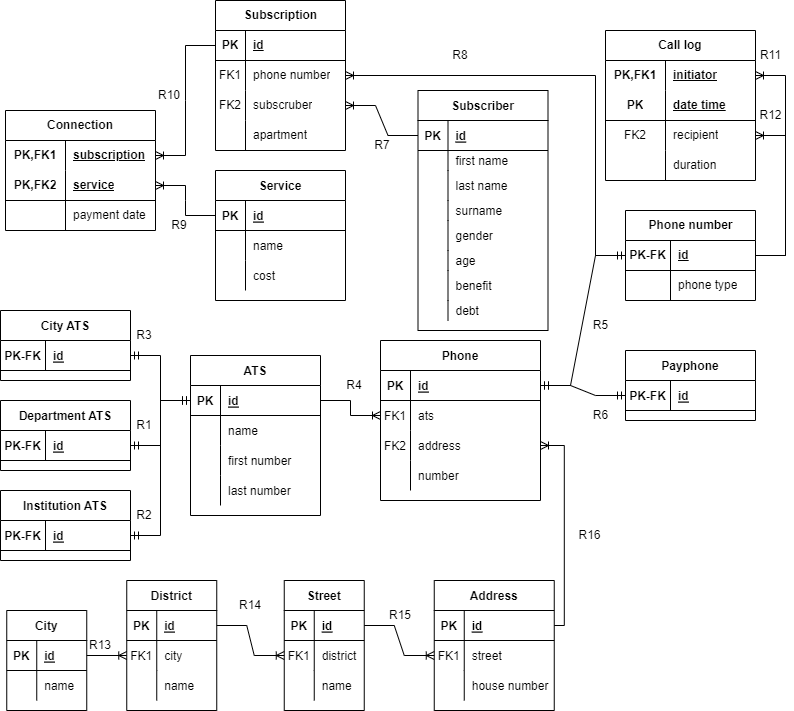
\includegraphics[width=\textwidth]{resources/er.png}
    \caption{ER диаграмма}
    \end{center}
\end{figure}

\end{document}
